\documentclass[a4paper,10pt,twoside]{article}

\usepackage[top=1in, bottom=1in, left=1in, right=1in]{geometry}
\usepackage[utf8]{inputenc}
\usepackage[spanish,es-ucroman,es-noquoting]{babel}
\usepackage{setspace}
\usepackage{fancyhdr}
\usepackage{lastpage}
\usepackage{amsmath}
\usepackage{amsfonts}
\usepackage{verbatim}
\usepackage{graphicx}
\usepackage{float}
\usepackage{algpseudocode}
\usepackage{enumitem} % Provee macro \setlist
\usepackage[toc, page]{appendix}


%%%%%%%%%% Configuración de Fancyhdr - Inicio %%%%%%%%%%
\pagestyle{fancy}
\thispagestyle{fancy}
\lhead{Trabajo Práctico 1 · Sistemas Operativos}
\rhead{Delgado · Lovisolo · Petaccio}
\renewcommand{\footrulewidth}{0.4pt}
\cfoot{\thepage /\pageref{LastPage}}

\fancypagestyle{caratula} {
   \fancyhf{}
   \cfoot{\thepage /\pageref{LastPage}}
   \renewcommand{\headrulewidth}{0pt}
   \renewcommand{\footrulewidth}{0pt}
}
%%%%%%%%%% Configuración de Fancyhdr - Fin %%%%%%%%%%


%%%%%%%%%% Configuración de Algorithmic - Inicio %%%%%%%%%%
% Entorno propio para customizar la presentación del pseudocódigo
\newenvironment{pseudo}[1][]{%
    \vspace{0.5em}%
    \begin{algorithmic}%
}
{%
    \end{algorithmic}%
    \vspace{0.5em}%
}

% Conectivo 'in' para usar así: \ForAll{$foo$ \In $bar$}
\newcommand{\In}{\textbf{in} }

% Conectivo 'to' para usar así: \For{$i = 1$ \In $n$}
\newcommand{\To}{\textbf{to} }

% Complejidades
\newcommand{\Ode}[1]{\hfill $O(#1)$}
%%%%%%%%%% Configuración de Algorithmic - Fin %%%%%%%%%%


%%%%%%%%%% Configuración de Appendix - Inicio %%%%%%%%%%
% Asigna la traducción de la palabra 'Appendices'.
\renewcommand{\appendixtocname}{Apéndices}
\renewcommand{\appendixpagename}{Apéndices}
%%%%%%%%%% Configuración de Appendix - Fin %%%%%%%%%%


%%%%%%%%%% Miscelánea - Inicio %%%%%%%%%%
% Evita que el documento se estire verticalmente para ocupar el espacio vacío
% en cada página.
\raggedbottom

% Deshabilita sangría en la primer línea de un párrafo.
\setlength{\parindent}{0em}

% Separación entre párrafos.
\setlength{\parskip}{0.5em}

% Separación entre elementos de listas.
\setlist{itemsep=0.5em}
%%%%%%%%%% Miscelánea - Fin %%%%%%%%%%


\begin{document}


%%%%%%%%%%%%%%%%%%%%%%%%%%%%%%%%%%%%%%%%%%%%%%%%%%%%%%%%%%%%%%%%%%%%%%%%%%%%%%%
%% Carátula                                                                  %%
%%%%%%%%%%%%%%%%%%%%%%%%%%%%%%%%%%%%%%%%%%%%%%%%%%%%%%%%%%%%%%%%%%%%%%%%%%%%%%%


\thispagestyle{caratula}

\begin{center}


\includegraphics[height=2cm]{DC.png} 
\hfill

\includegraphics[height=2cm]{UBA.jpg} 

\vspace{2cm}

Departamento de Computación,\\
Facultad de Ciencias Exactas y Naturales,\\
Universidad de Buenos Aires

\vspace{4cm}

\begin{Huge}
Trabajo Práctico 1
\end{Huge}

\vspace{0.5cm}

\begin{Large}
Sistemas Operativos
\end{Large}

\vspace{1cm}

Segundo Cuatrimestre de 2013

\vspace{4cm}

\begin{tabular}{|c|c|c|}
\hline
Apellido y Nombre & LU & E-mail\\
\hline
Alejandro Nahuel Delgado & 601/11 & nahueldelgado@gmail.com\\
Leandro Lovisolo      & 645/11 & leandro@leandro.me\\
Lautaro José Petaccio & 443/11 & lausuper@gmail.com\\
\hline
\end{tabular}

\end{center}

\newpage


%%%%%%%%%%%%%%%%%%%%%%%%%%%%%%%%%%%%%%%%%%%%%%%%%%%%%%%%%%%%%%%%%%%%%%%%%%%%%%%
%% Índice                                                                    %%
%%%%%%%%%%%%%%%%%%%%%%%%%%%%%%%%%%%%%%%%%%%%%%%%%%%%%%%%%%%%%%%%%%%%%%%%%%%%%%%


\tableofcontents

\newpage


%%%%%%%%%%%%%%%%%%%%%%%%%%%%%%%%%%%%%%%%%%%%%%%%%%%%%%%%%%%%%%%%%%%%%%%%%%%%%%%
%% Introducción                                                              %%
%%%%%%%%%%%%%%%%%%%%%%%%%%%%%%%%%%%%%%%%%%%%%%%%%%%%%%%%%%%%%%%%%%%%%%%%%%%%%%%


\section{Introducción}

Pendiente.


%%%%%%%%%%%%%%%%%%%%%%%%%%%%%%%%%%%%%%%%%%%%%%%%%%%%%%%%%%%%%%%%%%%%%%%%%%%%%%%
%% Ejercicio 1                                                               %%
%%%%%%%%%%%%%%%%%%%%%%%%%%%%%%%%%%%%%%%%%%%%%%%%%%%%%%%%%%%%%%%%%%%%%%%%%%%%%%%


\section{Ejercicio 1}

Pendiente.


%%%%%%%%%%%%%%%%%%%%%%%%%%%%%%%%%%%%%%%%%%%%%%%%%%%%%%%%%%%%%%%%%%%%%%%%%%%%%%%
%% Ejercicio 2                                                               %%
%%%%%%%%%%%%%%%%%%%%%%%%%%%%%%%%%%%%%%%%%%%%%%%%%%%%%%%%%%%%%%%%%%%%%%%%%%%%%%%


\section{Ejercicio 2}
El lote de tareas utilizado para el ejercicio es el siguiente:
\begin{pseudo}
	\State @0:
	\State TaskCPU 1000
	\State TaskConsola 3 100 200
	\State TaskConsola 5 150 270
\end{pseudo}

\begin{figure}[ht!]
\centering
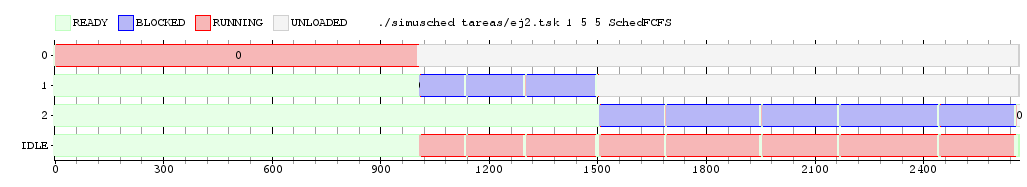
\includegraphics[width=175mm]{../ejercicio2/FCFS1Core.png}
\caption{Scheduler FCFS corriendo el lote de tareas con 1 core y 5 de penalidad por task switch}
\label{overflow}
\end{figure}

Puede observarse como el único core del scheduler para esta ejecución del simulador corre la tarea 0 hasta que esta se termina (1000 ticks).

Luego corre la tarea 1, la cuál realiza varios bloqueos y desbloqueos. Se puede notar el tiempo dedicado a hacer el task switch entre la tarea IDLE que corre mientras la tarea principal está bloqueada y la tarea principal.

Termina su ejecución con la tarea 2 que también realiza bloqueos y desbloqueos, intercambiando entre esta y su tarea IDLE.

\begin{figure}[ht!]
\centering
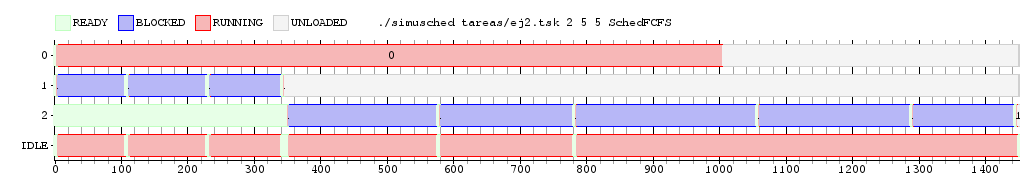
\includegraphics[width=175mm]{../ejercicio2/FCFS2Core.png}
\caption{Scheduler FCFS corriendo el lote de tareas con 2 core y 5 de penalidad por task switch}
\label{overflow}
\end{figure}

Puede observarse como en la figura 2, relacionada a la ejecución del simulador con 2 núcleos, como cada uno se comporta adecuadamente, tomando el core 0 la tarea 0, el core 1 la tarea 1 y ejecutándola hasta su finalización. Luego, como la tarea 1 finaliza antes que la 0, el core 0 toma la tarea 2 y la ejecuta.

\begin{figure}[ht!]
\centering
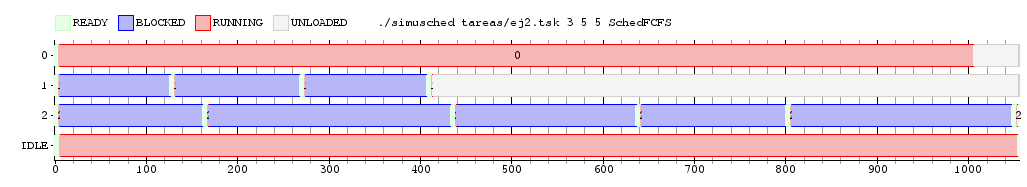
\includegraphics[width=175mm]{../ejercicio2/FCFS3Core.png}
\caption{Scheduler FCFS corriendo el lote de tareas con 3 core y 5 de penalidad por task switch}
\label{overflow}
\end{figure}

Observando la figura 3, puede notarse como cáda core toma cada una de las 3 tareas y las ejecuta simultáneamente hasta su finalización.

%%%%%%%%%%%%%%%%%%%%%%%%%%%%%%%%%%%%%%%%%%%%%%%%%%%%%%%%%%%%%%%%%%%%%%%%%%%%%%%
%% Ejercicio 3                                                               %%
%%%%%%%%%%%%%%%%%%%%%%%%%%%%%%%%%%%%%%%%%%%%%%%%%%%%%%%%%%%%%%%%%%%%%%%%%%%%%%%


\section{Ejercicio 3}

Pendiente.


%%%%%%%%%%%%%%%%%%%%%%%%%%%%%%%%%%%%%%%%%%%%%%%%%%%%%%%%%%%%%%%%%%%%%%%%%%%%%%%
%% Ejercicio 4                                                               %%
%%%%%%%%%%%%%%%%%%%%%%%%%%%%%%%%%%%%%%%%%%%%%%%%%%%%%%%%%%%%%%%%%%%%%%%%%%%%%%%


\section{Ejercicio 4}
El lote de tareas utilizado para la figura 4 es el siguiente:
\begin{pseudo}
	\State @0:
	\State TaskCPU 200
	\State TaskCPU 200
	\State TaskCPU 200
	\State TaskCPU 200
\end{pseudo}

Puede observarse en la figura 4 la ejecución del simulador con el Scheduler RoundRobin con 1 core con quantum 100 y penalidad de 5 para las task switch.

El gráfico muestra como las 4 tareas se ejecutan de forma cíclica, se ejecuta la tarea 0 a la 3 (haciendo cambio de tareas debido a que se les acaba el quantum) y se repite nuevamente este ciclo. Este comportamiento cíclcio de ejecución es el correspondiente al de un algoritmo de scheduling RoundRobin.

\begin{figure}[ht!]
\centering
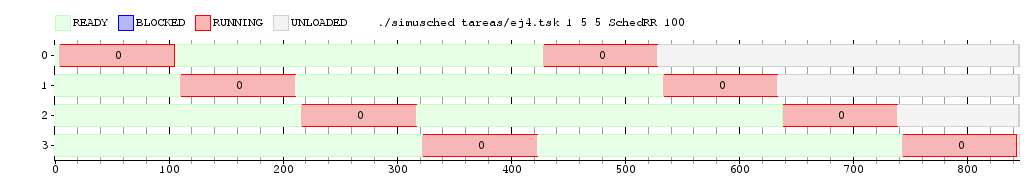
\includegraphics[width=175mm]{../ejercicio4/SchedRR1Core.png}
\caption{Scheduler RR corriendo el lote de tareas con 1 core con 100 de quantum y 5 de penalidad por task switch}
\label{overflow}
\end{figure}

El lote de tareas utilizado para la figura 5 es el siguiente:
\begin{pseudo}
	\State @0:
	\State TaskCPU 50
	\State TaskCPU 200
	\State TaskCPU 200
	\State TaskCPU 200
\end{pseudo}

Puede notarse nuevamente, en el gráfico de la figura 5, el cambio cíclico y ordenado de las tareas. En este caso, al tener una tarea de menor duración al inicio en el core 0, este queda asimétrico en relación al tiempo y a la ejecución de tareas, haciendo que en la próxima recorrida del ciclo del algoritmo, este tome las tareas del core 1, recibiendo una penalización de 50 ticks.

\begin{figure}[ht!]
\centering
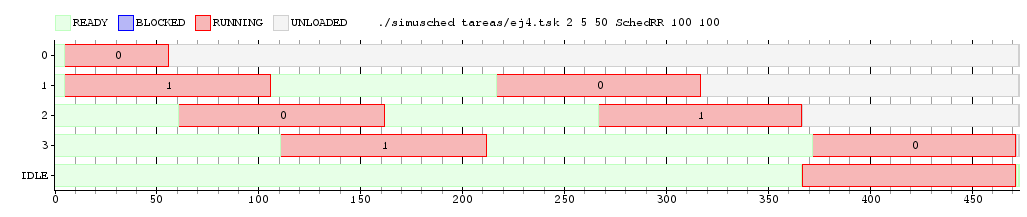
\includegraphics[width=175mm]{../ejercicio4/SchedRR2Core.png}
\caption{Scheduler RR corriendo el lote de tareas con 2 core de 100 de quantum cada uno y 50 de penalidad por task switch}
\label{overflow}
\end{figure}

El lote de tareas utilizado para la figura 6 es el siguiente:
\begin{pseudo}
	\State @0:
	\State TaskCPU 200
	\State TaskIO 50 400
	\State TaskCPU 200
	\State TaskCPU 200
\end{pseudo}

Por último, para demostrar la correctitud de la implementación del scheduler RoundRobin ante tareas bloqueantes, en la figura 6, puede verse como la tarea 1 se bloquea a los 50 ticks; el scheduler la remueve del ciclo continuando la ejecución las tareas sin tenerla en cuenta hasta que se realiza su desbloqueo, se agrega nuevamente al ciclo y termina.

\begin{figure}[ht!]
\centering
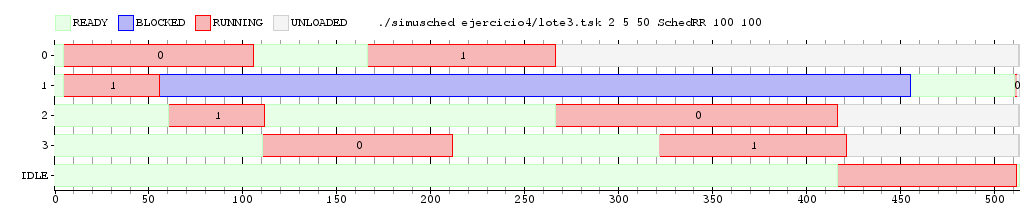
\includegraphics[width=175mm]{../ejercicio4/SchedRR2CoreIO.png}
\caption{Scheduler RR corriendo el lote de tareas con 2 core de 100 de quantum cada uno, 50 de penalidad por task switch y una tarea bloqueante}
\label{overflow}
\end{figure}

%%%%%%%%%%%%%%%%%%%%%%%%%%%%%%%%%%%%%%%%%%%%%%%%%%%%%%%%%%%%%%%%%%%%%%%%%%%%%%%
%% Ejercicio 5                                                               %%
%%%%%%%%%%%%%%%%%%%%%%%%%%%%%%%%%%%%%%%%%%%%%%%%%%%%%%%%%%%%%%%%%%%%%%%%%%%%%%%


\section{Ejercicio 5}

Pendiente.


%%%%%%%%%%%%%%%%%%%%%%%%%%%%%%%%%%%%%%%%%%%%%%%%%%%%%%%%%%%%%%%%%%%%%%%%%%%%%%%
%% Ejercicio 6                                                               %%
%%%%%%%%%%%%%%%%%%%%%%%%%%%%%%%%%%%%%%%%%%%%%%%%%%%%%%%%%%%%%%%%%%%%%%%%%%%%%%%


\section{Ejercicio 6}

Pendiente.


%%%%%%%%%%%%%%%%%%%%%%%%%%%%%%%%%%%%%%%%%%%%%%%%%%%%%%%%%%%%%%%%%%%%%%%%%%%%%%%
%% Ejercicio 7                                                               %%
%%%%%%%%%%%%%%%%%%%%%%%%%%%%%%%%%%%%%%%%%%%%%%%%%%%%%%%%%%%%%%%%%%%%%%%%%%%%%%%


\section{Ejercicio 7}

Pendiente.


%%%%%%%%%%%%%%%%%%%%%%%%%%%%%%%%%%%%%%%%%%%%%%%%%%%%%%%%%%%%%%%%%%%%%%%%%%%%%%%
%% Ejercicio 8                                                               %%
%%%%%%%%%%%%%%%%%%%%%%%%%%%%%%%%%%%%%%%%%%%%%%%%%%%%%%%%%%%%%%%%%%%%%%%%%%%%%%%


\section{Ejercicio 8}

Pendiente.


%%%%%%%%%%%%%%%%%%%%%%%%%%%%%%%%%%%%%%%%%%%%%%%%%%%%%%%%%%%%%%%%%%%%%%%%%%%%%%%
%% Ejercicio 9                                                               %%
%%%%%%%%%%%%%%%%%%%%%%%%%%%%%%%%%%%%%%%%%%%%%%%%%%%%%%%%%%%%%%%%%%%%%%%%%%%%%%%


\section{Ejercicio 9}

Pendiente.


%%%%%%%%%%%%%%%%%%%%%%%%%%%%%%%%%%%%%%%%%%%%%%%%%%%%%%%%%%%%%%%%%%%%%%%%%%%%%%%
%% Ejercicio 10                                                              %%
%%%%%%%%%%%%%%%%%%%%%%%%%%%%%%%%%%%%%%%%%%%%%%%%%%%%%%%%%%%%%%%%%%%%%%%%%%%%%%%


\section{Ejercicio 10}

Pendiente.


%%%%%%%%%%%%%%%%%%%%%%%%%%%%%%%%%%%%%%%%%%%%%%%%%%%%%%%%%%%%%%%%%%%%%%%%%%%%%%%
%% Conclusiones                                                              %%
%%%%%%%%%%%%%%%%%%%%%%%%%%%%%%%%%%%%%%%%%%%%%%%%%%%%%%%%%%%%%%%%%%%%%%%%%%%%%%%


\section{Conclusiones}

Pendiente.


%%%%%%%%%%%%%%%%%%%%%%%%%%%%%%%%%%%%%%%%%%%%%%%%%%%%%%%%%%%%%%%%%%%%%%%%%%%%%%%
%% Apéndice                                                                  %%
%%%%%%%%%%%%%%%%%%%%%%%%%%%%%%%%%%%%%%%%%%%%%%%%%%%%%%%%%%%%%%%%%%%%%%%%%%%%%%%

\newpage

\begin{appendices}

\section{Apéndice}

Pendiente.


\end{appendices}

\end{document}